%==============================================================================
%  GoPlus — Technical Project Report
%  Formal template, HUST red/white tone. Compiles with pdflatex (twice).
%  Fill the placeholders on the title page and drop a `logo.png` next to this
%  file to show the university logo.
%==============================================================================
\documentclass[11pt,a4paper]{article}

\usepackage[T1]{fontenc}
\usepackage[utf8]{inputenc}
\usepackage{lmodern}
\usepackage{inconsolata} % robust, complete monospace font for code listings
\usepackage{microtype}
\usepackage[a4paper,margin=2.5cm,headheight=15pt]{geometry}
\usepackage{graphicx}
\usepackage{xcolor}
\usepackage{titlesec}
\usepackage{fancyhdr}
\usepackage{booktabs}
\usepackage{tabularx}
\usepackage{array}
\usepackage{enumitem}
\usepackage{caption}
\usepackage{listings}
\usepackage{tikz}
\usetikzlibrary{positioning,arrows.meta,shapes.geometric,calc}
\usepackage{pgfplots}
\pgfplotsset{compat=1.18}
\usepackage[colorlinks=true]{hyperref}

%------------------------------------------------------------------ HUST colours
\definecolor{hustred}{HTML}{A31621}   % dignified deep crimson (adjust to brand)
\definecolor{hustdark}{HTML}{5C0A14}  % darker accent for headings/links
\definecolor{codebg}{HTML}{FBF7F7}    % faint warm-white code background
\definecolor{codegray}{HTML}{6E6E6E}
\definecolor{codestr}{HTML}{2A6F5A}

\hypersetup{linkcolor=hustdark,urlcolor=hustred,citecolor=hustdark}

%------------------------------------------------------------------ section look
\titleformat{\section}
  {\Large\bfseries\color{hustred}}{\thesection}{0.6em}{}
  [{\vspace{-0.4ex}{\color{hustred}\titlerule[1.1pt]}}]
\titleformat{\subsection}
  {\large\bfseries\color{hustdark}}{\thesubsection}{0.5em}{}
\titlespacing*{\section}{0pt}{2.2ex plus .2ex}{1.2ex}

%------------------------------------------------------------------ headers
\pagestyle{fancy}
\fancyhf{}
\fancyhead[L]{\small\color{hustdark}\textbf{GoPlus}\;\textcolor{hustred}{\textbar}\; A Productivity Layer for Go}
\fancyhead[R]{\small\color{hustdark}Technical Report}
\fancyfoot[C]{\small\color{hustdark}\thepage}
\renewcommand{\headrulewidth}{0pt}
\renewcommand{\headrule}{\hbox to\headwidth{\color{hustred}\leaders\hrule height 1pt\hfill}}
\renewcommand{\footrulewidth}{0pt}

%------------------------------------------------------------------ code styling
\lstdefinelanguage{GoPlus}{
  morekeywords={fn,func,struct,enum,impl,match,return,if,else,for,switch,select,%
    defer,go,const,var,mut,self,type,package,import,range,chan,map,interface,true,false,nil},
  morekeywords=[2]{String,Debug,Equal,Clone,JsonMarshal,JsonUnmarshal,JSON,derive,log,retry,memoize},
  sensitive=true,
  morecomment=[l]{//},
  morecomment=[s]{/*}{*/},
  morestring=[b]",
  morestring=[b]`,
}
\lstdefinelanguage{Golang}{
  morekeywords={func,package,import,if,else,for,switch,case,default,return,var,%
    const,type,struct,interface,range,chan,map,defer,go,select,nil,error,true,false},
  sensitive=true,
  morecomment=[l]{//},
  morecomment=[s]{/*}{*/},
  morestring=[b]",
  morestring=[b]`,
}
\lstdefinestyle{gp}{
  language=GoPlus,
  basicstyle=\ttfamily\small,
  keywordstyle=\color{hustred}\bfseries,
  keywordstyle=[2]\color{hustdark}\bfseries,
  commentstyle=\color{codegray}\itshape,
  stringstyle=\color{codestr},
  backgroundcolor=\color{codebg},
  frame=single,
  rulecolor=\color{hustred!55},
  framesep=6pt,
  xleftmargin=10pt,xrightmargin=6pt,
  aboveskip=1.1em,belowskip=0.6em,
  showstringspaces=false,
  breaklines=true,
  columns=fullflexible,
  keepspaces=true,
}
\lstset{style=gp}
\newcommand{\gofile}[1]{\lstset{style=gp,language=Golang}#1\lstset{style=gp,language=GoPlus}}

\captionsetup{font=small,labelfont={bf,color=hustdark}}
\setlength{\parskip}{0.35em}
\setlength{\parindent}{0pt}

%==============================================================================
\begin{document}

%---------------------------------------------------------------- TITLE PAGE
\begin{titlepage}
\thispagestyle{empty}
\centering
{\color{hustred}\rule{\textwidth}{2pt}}\\[1.2ex]
{\large\bfseries HANOI UNIVERSITY OF SCIENCE AND TECHNOLOGY}\\[0.4ex]
{\normalsize \emph{$\langle$ School / Faculty placeholder $\rangle$}}\\[2.2ex]

\IfFileExists{logo.png}
  {
\includegraphics[height=2.8cm]{logo.png}}
  {\setlength{\fboxrule}{1pt}\setlength{\fboxsep}{0pt}%
   \textcolor{hustred}{\fbox{\parbox[c][2.8cm][c]{2.8cm}{\centering\small\itshape drop\\ logo.png\\ here}}}}

\vfill
{\color{hustred}\rule{0.85\textwidth}{0.8pt}}\\[2.4ex]
{\Huge\bfseries\color{hustred} GoPlus}\\[1.0ex]
{\LARGE\bfseries A Productivity Layer for Go}\\[1.2ex]
{\large A source-language and Rust transpiler that keeps Go transparent}\\[2.4ex]
{\color{hustred}\rule{0.85\textwidth}{0.8pt}}
\vfill

\begin{tabular}{@{}r@{\hskip 1.2em}l@{}}
\textbf{Author}      & $\langle$ Full name $\rangle$ \\
\textbf{Student ID}  & $\langle$ ID $\rangle$ \\
\textbf{Programme}   & $\langle$ Programme / Major $\rangle$ \\
\textbf{Supervisor}  & $\langle$ Supervisor $\rangle$ \\
\textbf{Course}      & $\langle$ Course / Subject $\rangle$ \\
\textbf{Date}        & $\langle$ Month, Year $\rangle$ \\
\end{tabular}

\vspace{1.6em}
{\color{hustred}\rule{\textwidth}{2pt}}
\end{titlepage}

%---------------------------------------------------------------- ABSTRACT + TOC
\pagenumbering{roman}
\section*{\centering\color{hustred} Abstract}
\addcontentsline{toc}{section}{Abstract}
\begin{quote}\itshape
GoPlus is a surface language for Go, implemented as a transpiler that turns
\texttt{.gp} sources into ordinary \texttt{.go} files. It preserves the entire Go
ecosystem---toolchain, runtime, and packages---while sharpening the developer
experience: concise error propagation, first-class enumerations with exhaustive
pattern matching, and safe compile-time decorators. A central design constraint
is that the generated Go stays readable and idiomatic, so teams retain full
transparency and incur no lock-in. This report presents the motivation, design
philosophy, language surface, compiler architecture, and developer tooling of
GoPlus, and evaluates it against hand-written Go. On representative patterns the
same behaviour is expressed in roughly 40--80\% fewer tokens, while the generated
code runs at parity with hand-written Go (measured at zero additional
allocations), and transpilation completes in micro- to milliseconds. A small
REST service written entirely in GoPlus demonstrates the approach on a
medium-sized, real program.
\end{quote}
\vspace{0.5em}
\noindent\textbf{Keywords:} Go, transpiler, developer experience, error handling,
algebraic enumerations, pattern matching, compile-time metaprogramming.

\vspace{1.5em}
{\color{hustred}\hrulefill}
\tableofcontents
\vspace{1em}
{\color{hustred}\hrulefill}
\clearpage
\pagenumbering{arabic}

%================================================================ 1
\section{Introduction and Motivation}
Go is prized for its simplicity, fast compilation, first-class concurrency, and
an exceptional standard toolchain. That same minimalism, however, leaves
recurring ergonomic gaps in everyday application code. Three stand out.

\begin{itemize}[leftmargin=1.4em,itemsep=0.2em]
  \item \textbf{Verbose error flow.} The idiomatic \texttt{if err != nil} check,
        repeated after nearly every fallible call, dominates the visual weight of
        real code and obscures the intended logic.
  \item \textbf{No exhaustive enumerations.} A set of states is usually modelled
        with \texttt{const}/\texttt{iota} and a \texttt{switch}; the compiler
        cannot tell the developer when a new state is left unhandled.
  \item \textbf{No safe metaprogramming.} Cross-cutting concerns such as
        logging, retrying, or memoizing a function are written by hand at every
        call site, or bolted on with reflection.
\end{itemize}

GoPlus addresses these gaps with a \emph{thin surface layer} that compiles down
to ordinary Go. It is deliberately \emph{not} a new language runtime and \emph{not}
a replacement for Go: it is a productivity layer whose output is plain,
\texttt{gofmt}-formatted Go that any Go developer can read, review, and debug.

A second, increasingly relevant motivation is the cost of writing code with AI
assistants. Because a large-language-model's effort and price scale with the
number of tokens produced, a more concise yet unambiguous surface language lets
an agent express the same behaviour with fewer tokens and fewer opportunities to
get boilerplate wrong. Section~\ref{sec:eval} quantifies this effect.

\paragraph{Contributions.} This report describes: (i) the design goals that keep
GoPlus compatible and transparent; (ii) the language surface for error handling,
enumerations and matching, decorators, and derivations; (iii) a straight-line
compiler architecture that keeps the generated Go idiomatic; (iv) the developer
tooling (formatter, linter, diagnostics, editor support); and (v) an evaluation
against hand-written Go, including a medium-sized case study.

%================================================================ 2
\section{Design Goals and Non-Goals}
GoPlus is defined as much by what it refuses to do as by what it adds. Keeping
the scope small is what allows the generated Go to stay clean.

\begin{table}[h]
\centering
\renewcommand{\arraystretch}{1.25}
\begin{tabularx}{\textwidth}{@{}p{0.46\textwidth} X@{}}
\toprule
\textbf{\color{hustred}Goals} & \textbf{\color{hustred}Non-goals} \\
\midrule
Practical compatibility with the Go toolchain &
A borrow checker or ownership system \\
A low learning curve --- standard Go syntax is also accepted &
A free-form, token-level macro system \\
Concise error handling via \texttt{!} and \texttt{?} &
A custom runtime replacing the Go runtime \\
Strong enum/match support with exhaustiveness &
An overly complex type system that hurts simplicity \\
Flexible compile-time decorators, incl.\ user-defined ones & \\
Human-readable output, always \texttt{gofmt}-formatted & \\
\bottomrule
\end{tabularx}
\caption{The scope of GoPlus, stated as goals and explicit non-goals.}
\end{table}

The overarching principle is \emph{transparency}: every construct must lower to
Go that a person could plausibly have written by hand. This keeps the project
free of lock-in---a team can, at any point, take the generated Go and walk away.

%================================================================ 3
\section{Language Overview}
This section introduces the surface features at a conceptual level. The examples
are illustrative; the point is the shape of the syntax and what it means, not any
particular implementation detail.

\subsection{Concise error handling}
A function that can fail declares its result with a trailing \texttt{!}
(\texttt{-> T!} for ``a \texttt{T} or an error'', \texttt{-> !} for
``possibly an error''). The postfix \texttt{?} operator propagates an error from
a fallible call, so the happy path reads top to bottom.

\begin{lstlisting}[language=GoPlus,caption={Error propagation in GoPlus.}]
fn loadConfig(path: string) -> Config! {
    raw    := readFile(path)?
    parsed := parse(raw)?
    return validate(parsed)?
}
\end{lstlisting}

Conceptually, each \texttt{?} expands to the familiar Go check---capture the
value and error, and return early on failure---so the emitted Go is exactly the
code a developer would otherwise write, only generated automatically:

\begin{lstlisting}[language=Golang,caption={The Go that the previous example stands in for.}]
func loadConfig(path string) (Config, error) {
    raw, err := readFile(path)
    if err != nil { return Config{}, err }
    parsed, err := parse(raw)
    if err != nil { return Config{}, err }
    return validate(parsed)
}
\end{lstlisting}

The semantic layer only permits \texttt{?} inside a function whose result can
carry an error, so misuse is caught at compile time rather than surfacing as a
confusing Go error later.

\subsection{Enumerations and exhaustive matching}
GoPlus offers both simple enumerations and tagged (payload-carrying, optionally
generic) enumerations, together with a \texttt{match} expression that the
compiler checks for exhaustiveness. Forgetting a case is a compile error, so a
newly added variant cannot silently slip through.

\begin{lstlisting}[language=GoPlus,caption={An enum state machine with an exhaustive match.}]
@derive(String)
enum Status { Todo  InProgress  Done  Cancelled }

fn canAdvance(from: Status, to: Status) -> bool {
    match from {
        Todo       => to == Status::InProgress || to == Status::Cancelled
        InProgress => to == Status::Done       || to == Status::Cancelled
        Done       => false
        Cancelled  => false
    }
}
\end{lstlisting}

A simple enum lowers to an integer type with named constants and a generated
\texttt{String()} method; a \texttt{match} lowers to a Go \texttt{switch}. The
difference from writing the \texttt{switch} by hand is that GoPlus \emph{enforces}
that every variant is handled---an assurance the Go compiler does not provide.

Tagged enumerations carry data and may be generic. They express a result or a
sum type directly, and \texttt{match} binds the payload:

\begin{lstlisting}[language=GoPlus,caption={A generic tagged enumeration.}]
enum Result<T> {
    Ok(T)
    Err(string)
}

fn describe(r: Result<int>) -> string {
    match r {
        Ok(value)  => fmt.Sprintf("ok: %d", value)
        Err(reason) => "error: " + reason
    }
}
\end{lstlisting}

A tagged enum lowers to a small tagged \texttt{struct} with constructor functions
and Go generics, so it too remains ordinary, inspectable Go.

\subsection{Compile-time decorators}
Cross-cutting behaviour is attached with decorators. Built-in decorators cover
common needs---\texttt{@log}, \texttt{@retry}, \texttt{@memoize}---and users can
define their own following a small, Python-like contract (a decorator receives
the next function in the chain and returns a wrapped function with the same
signature).

\begin{lstlisting}[language=GoPlus,caption={Decorators replace hand-rolled wrappers.}]
@log
@retry(3, 10)
fn fetch(id: int) -> Payload! {
    return callService(id)?
}
\end{lstlisting}

Each decorator is expanded at compile time into a named wrapper function, so the
resulting Go is ordinary, inspectable code---there is no reflection and no
runtime indirection. The semantic layer validates that a custom decorator's
signature is compatible with the function it wraps.

\begin{figure}[ht]
\centering
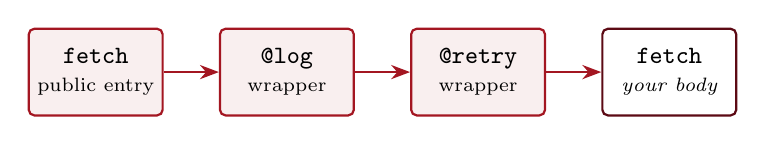
\begin{tikzpicture}[
  node distance=7mm,
  b/.style={draw=hustred,fill=hustred!7,rounded corners=2pt,thick,minimum height=11mm,
            minimum width=17mm,align=center,font=\small,inner sep=3pt},
  bi/.style={draw=hustdark,fill=white,rounded corners=2pt,thick,minimum height=11mm,
             minimum width=17mm,align=center,font=\small,inner sep=3pt},
  a/.style={-{Stealth[length=2.4mm]},hustred,thick}]
\node[b] (pub) {\texttt{fetch}\\[-1pt]{\scriptsize public entry}};
\node[b,right=of pub] (log) {\texttt{@log}\\[-1pt]{\scriptsize wrapper}};
\node[b,right=of log] (retry) {\texttt{@retry}\\[-1pt]{\scriptsize wrapper}};
\node[bi,right=of retry] (inner) {\texttt{fetch}\\[-1pt]{\scriptsize \itshape your body}};
\draw[a] (pub)--(log);
\draw[a] (log)--(retry);
\draw[a] (retry)--(inner);
\end{tikzpicture}
\caption{\texttt{@log @retry fn fetch} compiles to a chain of named wrapper
functions: a call enters at the public \texttt{fetch} and unwinds inward to your
body. The first decorator listed becomes the outermost wrapper.}
\label{fig:decor}
\end{figure}

\subsection{Derivations}
The \texttt{@derive} annotation generates routine methods so they need not be
written and maintained by hand: \texttt{String}, \texttt{Debug}, \texttt{Equal},
\texttt{Clone}, and JSON (de)serialization.

\begin{lstlisting}[language=GoPlus,caption={Deriving boilerplate methods.}]
@derive(JsonMarshal, JsonUnmarshal, Clone)
struct Task {
    ID:    int     `json:"id"`
    Title: string  `json:"title"`
    State: Status  `json:"state"`
}
\end{lstlisting}

Notably, the derived \texttt{Clone} performs a \emph{deep} copy of slice and map
fields, avoiding a subtle and common Go bug in which a value copy silently shares
the underlying storage. JSON derivations honour explicit field tags.

\subsection{Interoperability}
GoPlus is designed to sit inside real Go projects. Standard Go syntax is accepted
alongside the GoPlus surface, a package may mix \texttt{.gp} and \texttt{.go}
files that link together, and the standard library is used directly. Nothing about
adopting GoPlus removes the option of dropping back to plain Go.

\subsection{The surface at a glance}
Table~\ref{tab:glance} summarises how each concern is expressed in GoPlus versus
plain Go. In every row the GoPlus form is not only shorter but also carries a
guarantee the plain-Go form lacks.

\begin{table}[ht]
\centering
\renewcommand{\arraystretch}{1.3}
\begin{tabularx}{\textwidth}{@{}p{0.24\textwidth} X X@{}}
\toprule
\textbf{\color{hustred}Concern} & \textbf{\color{hustred}GoPlus} & \textbf{\color{hustred}Plain Go} \\
\midrule
Error propagation & \texttt{x := f()?} in a \texttt{->\,T!} function &
  \texttt{x, err := f(); if err != nil \{ return \}} at every call \\
Finite state set & \texttt{enum} + exhaustive \texttt{match} (compiler-checked) &
  \texttt{const}/\texttt{iota} + \texttt{switch} (unchecked) \\
Cross-cutting behaviour & a decorator, e.g.\ \texttt{@retry(3)} &
  a hand-written wrapper function \\
Routine methods & \texttt{@derive(String, Equal, Clone, JSON)} &
  written and maintained by hand \\
Safe deep copy & \texttt{@derive(Clone)} copies slices/maps &
  a value copy silently shares backing storage \\
\bottomrule
\end{tabularx}
\caption{Each concern, expressed in GoPlus and in plain Go.}
\label{tab:glance}
\end{table}

%================================================================ 4
\section{Compiler Architecture}
GoPlus is a straight-line transpiler. Each stage has a single responsibility, and
the last two stages hand off to the unmodified Go toolchain.

\begin{figure}[h]
\centering
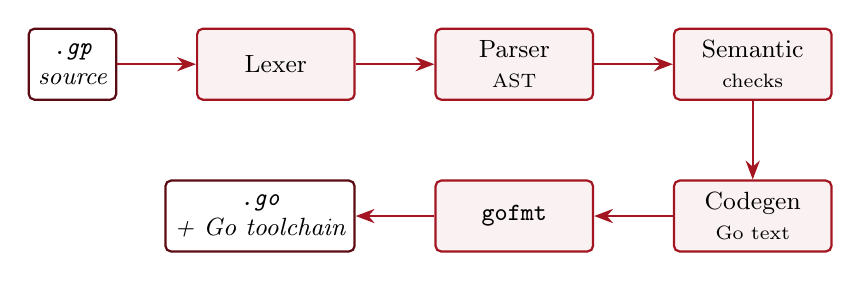
\begin{tikzpicture}[
  node distance=8mm and 10mm,
  box/.style={draw=hustred,fill=hustred!6,rounded corners=2pt,thick,
              minimum height=9mm,minimum width=20mm,align=center,font=\small},
  io/.style={draw=hustdark,fill=white,rounded corners=2pt,thick,
             minimum height=9mm,align=center,font=\small\itshape},
  arr/.style={-{Stealth[length=2.4mm]},hustred,thick}]
\node[io] (src) {\texttt{.gp}\\ source};
\node[box,right=of src] (lex) {Lexer};
\node[box,right=of lex] (par) {Parser\\{\scriptsize AST}};
\node[box,right=of par] (sem) {Semantic\\{\scriptsize checks}};
\node[box,below=10mm of sem] (cod) {Codegen\\{\scriptsize Go text}};
\node[box,left=of cod] (fmt) {\texttt{gofmt}};
\node[io,left=of fmt] (go) {\texttt{.go}\\ + Go toolchain};
\draw[arr] (src)--(lex);
\draw[arr] (lex)--(par);
\draw[arr] (par)--(sem);
\draw[arr] (sem)--(cod);
\draw[arr] (cod)--(fmt);
\draw[arr] (fmt)--(go);
\end{tikzpicture}
\caption{The GoPlus pipeline: lex \(\rightarrow\) parse \(\rightarrow\) analyze
\(\rightarrow\) generate \(\rightarrow\) format \(\rightarrow\) Go toolchain.}
\end{figure}

\begin{description}[leftmargin=1.4em,style=nextline]
  \item[Lexer] converts source into a token stream.
  \item[Parser] builds an abstract syntax tree. Language constructs
        (declarations, \texttt{if}/\texttt{else}, \texttt{match}, and the control-flow
        statements \texttt{for}/\texttt{switch}/\texttt{select}) are parsed into
        structured nodes; a few line-level constructs are kept as verbatim
        pass-through. Unfamiliar shapes fall back to raw text rather than failing
        the whole file.
  \item[Semantic layer] enforces the guarantees that make GoPlus safe:
        exhaustive \texttt{match}, valid \texttt{?} context, decorator contracts,
        and duplicate/collision checks. It descends into every block---including
        the bodies of loops and switches---so nested constructs are analyzed at
        any depth.
  \item[Codegen] emits deliberately readable Go: enums become integer or tagged
        struct types, \texttt{match} becomes a \texttt{switch}, \texttt{?} becomes
        an explicit error check, and \texttt{@derive} emits the corresponding
        methods.
  \item[\texttt{gofmt}] formats the generated Go, so the output reads like code a
        person wrote.
\end{description}

Figure~\ref{fig:desugar} sketches how three surface constructs are lowered. In
every case the result is plain Go with no hidden machinery.

\begin{figure}[ht]
\centering
\renewcommand{\arraystretch}{1.5}
\begin{tabular}{@{}p{0.40\textwidth} c p{0.44\textwidth}@{}}
\toprule
\multicolumn{1}{@{}l}{\textbf{\color{hustred}GoPlus construct}} & &
\multicolumn{1}{l@{}}{\textbf{\color{hustred}generated Go (in essence)}} \\
\midrule
\texttt{x := f()?} & \textcolor{hustred}{\large$\Rightarrow$} &
  \texttt{x, err := f()}\newline\texttt{if err != nil \{ return z, err \}} \\
\texttt{match s \{ A => e \}} & \textcolor{hustred}{\large$\Rightarrow$} &
  \texttt{switch s \{ case A: return e \}} \\
\texttt{@memoize fn g(n)} & \textcolor{hustred}{\large$\Rightarrow$} &
  \texttt{g\_inner + guarded cache + g} \\
\bottomrule
\end{tabular}
\caption{Representative desugarings. Each surface construct lowers to plain,
idiomatic Go; nothing is added at run time beyond what the construct means.}
\label{fig:desugar}
\end{figure}

\subsection{Semantic guarantees}
The value of the semantic layer is that it turns whole classes of latent bugs
into compile-time errors, close to where the developer is working rather than
deep inside a generated Go file:
\begin{itemize}[leftmargin=1.4em,itemsep=0.2em]
  \item \textbf{Exhaustiveness.} A \texttt{match} over an enumeration must handle
        every variant (or use an explicit wildcard); adding a variant makes any
        incomplete match fail to compile.
  \item \textbf{Error context.} The \texttt{?} operator is only accepted in a
        function whose result can carry an error, so it can never expand into
        invalid Go.
  \item \textbf{Decorator contracts.} A custom decorator is checked against the
        signature of the function it wraps, on both free functions and methods.
  \item \textbf{Name integrity.} Duplicate declarations and collisions with the
        compiler's generated names are detected before code generation.
\end{itemize}
Because analysis descends into every nested block, these checks hold at any
depth---for example, for a \texttt{match} written inside a loop or a switch case.

\subsection{Transparency, source maps, and incremental builds}
Two properties keep GoPlus practical at scale. First, the generated Go is always
run through \texttt{gofmt} and is written to read like hand-authored code, so it
can be reviewed, stepped through in a debugger, and---if ever necessary---kept as
the project's own source. Second, two facilities support tooling:
\emph{source maps} record \texttt{.gp}\,\(\leftrightarrow\)\,\texttt{.go} ranges
for declarations, functions, match arms, and statements, enabling bidirectional
``go to definition''; and a \emph{content-hash package cache} lets incremental
builds skip packages whose sources have not changed, keeping continuous-integration
loops fast.

\begin{figure}[ht]
\centering
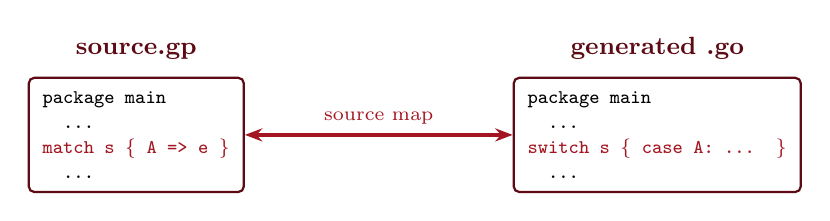
\begin{tikzpicture}[
  side/.style={draw=hustdark,rounded corners=2pt,thick,align=left,
               font=\ttfamily\scriptsize,inner sep=5pt,fill=white},
  a/.style={{Stealth[length=2.2mm]}-{Stealth[length=2.2mm]},hustred,very thick}]
\node[side] (gp) {package main\\[1pt]\ \ ...\\[1pt]\textcolor{hustred}{match s \{ A => e \}}\\[1pt]\ \ ...};
\node[side,right=34mm of gp] (go) {package main\\[1pt]\ \ ...\\[1pt]\textcolor{hustred}{switch s \{ case A: ... \}}\\[1pt]\ \ ...};
\node[above=1mm of gp,font=\small\bfseries\color{hustdark}] {source.gp};
\node[above=1mm of go,font=\small\bfseries\color{hustdark}] {generated .go};
\draw[a] (gp.east) -- node[above,font=\scriptsize\color{hustred}]{source map} (go.west);
\end{tikzpicture}
\caption{A source map records \texttt{.gp}\,$\leftrightarrow$\,\texttt{.go}
ranges, so an editor can jump in either direction---from a GoPlus construct to
the Go it produced, and back.}
\label{fig:srcmap}
\end{figure}

\subsection{Implementation footprint}
The compiler is a modestly-sized Rust codebase---roughly nine thousand lines of
implementation---partitioned so that no component grows into a catch-all.
Figure~\ref{fig:loc} shows the distribution; code generation is the largest, as
befits the stage that must emit idiomatic Go for every construct. The project is
backed by 80 unit and integration tests and 18 runnable examples.

\begin{figure}[ht]
\centering
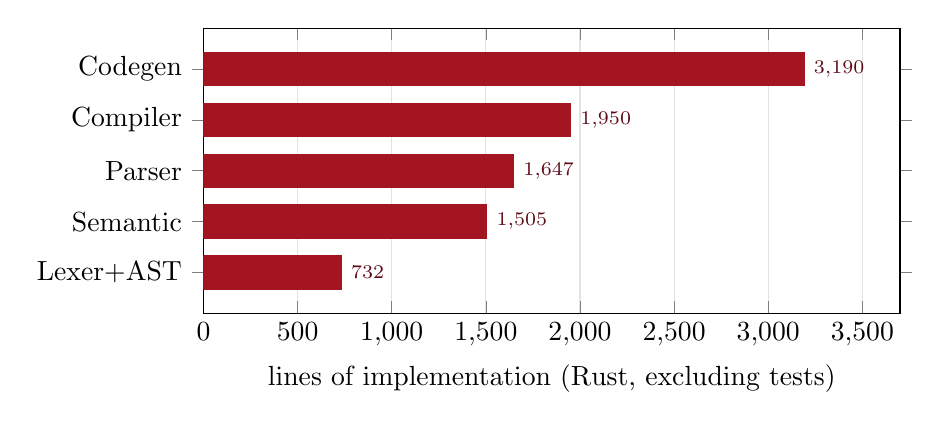
\begin{tikzpicture}
\begin{axis}[
  xbar, bar width=12pt,
  width=0.86\textwidth, height=5.2cm,
  xmin=0, xmax=3700,
  xlabel={lines of implementation (Rust, excluding tests)},
  symbolic y coords={{Lexer+AST}, Semantic, Parser, Compiler, Codegen},
  ytick=data,
  nodes near coords, nodes near coords style={font=\scriptsize\color{hustdark}},
  enlarge y limits=0.2,
  xmajorgrids, grid style={gray!22},
]
\addplot[fill=hustred,draw=hustred] coordinates {
  (3190,Codegen) (1950,Compiler) (1647,Parser) (1505,Semantic) (732,{Lexer+AST})
};
\end{axis}
\end{tikzpicture}
\caption{Implementation size by component. The frontend, semantic layer, code
generator, and project orchestration are cleanly separated.}
\label{fig:loc}
\end{figure}

%================================================================ 5
\section{Developer Tooling and Experience}
A language layer is only as good as the tooling around it. GoPlus ships a
coherent set of developer tools built on the same frontend.

\begin{itemize}[leftmargin=1.4em,itemsep=0.25em]
  \item \textbf{Formatter.} A rewriting formatter reproduces a canonical form of
        each source file. It is \emph{comment-preserving} and \emph{idempotent},
        and it is safe by construction: rather than risk dropping a comment, it
        declines to overwrite a file it cannot format losslessly.
  \item \textbf{Linter.} A set of stably-coded rules flag stylistic and
        suspicious-code issues without generating Go---for example, an
        unreachable arm after a wildcard, or a wildcard that quietly defeats the
        exhaustiveness of an enum match.
  \item \textbf{Diagnostics.} Errors and warnings carry a stable code, a precise
        caret span, and an actionable hint, and are available in a
        machine-readable form for editors.
  \item \textbf{Editor support.} A first-party editor extension provides syntax
        highlighting, inline diagnostics, hover documentation, snippets,
        format-on-save, and source navigation between \texttt{.gp} and the
        generated \texttt{.go}.
\end{itemize}

\subsection{Linting}
The linter reports issues that the type system alone would not, each under a
stable code so they can be tracked and suppressed deliberately.
Table~\ref{tab:lint} lists the current rules.

\begin{table}[ht]
\centering
\renewcommand{\arraystretch}{1.2}
\begin{tabularx}{\textwidth}{@{}l X@{}}
\toprule
\textbf{\color{hustred}Code} & \textbf{\color{hustred}Detects} \\
\midrule
\texttt{L0001} & An imported package that is never used \\
\texttt{L0002} & A type or function name that breaks the naming convention \\
\texttt{L0003} & An empty function body \\
\texttt{L0004} & A redundant trailing \texttt{return} in a void function \\
\texttt{L0005} & An unreachable match arm following a wildcard \\
\texttt{L0006} & A function large enough to warrant refactoring \\
\texttt{L0007} & An enum used in formatting without a derived \texttt{String} \\
\texttt{L0008} & A wildcard that hides unlisted enum variants, defeating exhaustiveness \\
\bottomrule
\end{tabularx}
\caption{Linter rules, each with a stable diagnostic code.}
\label{tab:lint}
\end{table}

\subsection{Diagnostics}
Every diagnostic carries a severity, a stable code, a precise caret span, and an
actionable hint. A human-readable rendering looks like the following, and the
same information is available as structured JSON for editors and other tools:

\begin{lstlisting}[language=GoPlus,caption={A diagnostic with code, span, and hint.}]
warning L0008: `_` in this match on enum `Color` hides 2 unlisted
               variant(s): Green, Blue
    match c {
    ^^^^^^^^^
hint: list the variants explicitly so exhaustiveness catches new ones
\end{lstlisting}

%================================================================ 6
\section{Evaluation}\label{sec:eval}
Three small, reproducible benchmarks test the project's central claims: that
GoPlus reduces the amount of code written, that it adds no runtime cost, and that
it transpiles quickly. Each measures the \emph{same behaviour} implemented two
ways where a comparison applies.

\subsection{Token economy}
For five representative patterns, the same program was written once in GoPlus
and once in plain hand-written Go. Token counts use a modern LLM tokenizer.

\begin{table}[h]
\centering
\renewcommand{\arraystretch}{1.2}
\begin{tabularx}{\textwidth}{@{}X r r r@{}}
\toprule
\textbf{Pattern} & \textbf{GoPlus (tok.)} & \textbf{Hand Go (tok.)} & \textbf{Reduction} \\
\midrule
Error-propagation chain (\texttt{?})     &  81 & 130 & \textbf{--38\%} \\
Enum state machine + \texttt{String}     &  69 & 151 & \textbf{--54\%} \\
Struct equality/debug derive             &  30 &  94 & \textbf{--68\%} \\
JSON model derive                        &  61 & 244 & \textbf{--75\%} \\
Decorated API call (retry + log)         &  40 & 188 & \textbf{--79\%} \\
\midrule
\textbf{Total}                           & \textbf{281} & \textbf{807} & \textbf{--65\%} \\
\bottomrule
\end{tabularx}
\caption{The same behaviour uses substantially fewer tokens in GoPlus. The saving
grows with the amount of boilerplate replaced---derivations and decorators, which
stand in for whole method bodies and wrappers, save the most.}
\end{table}

\begin{figure}[ht]
\centering
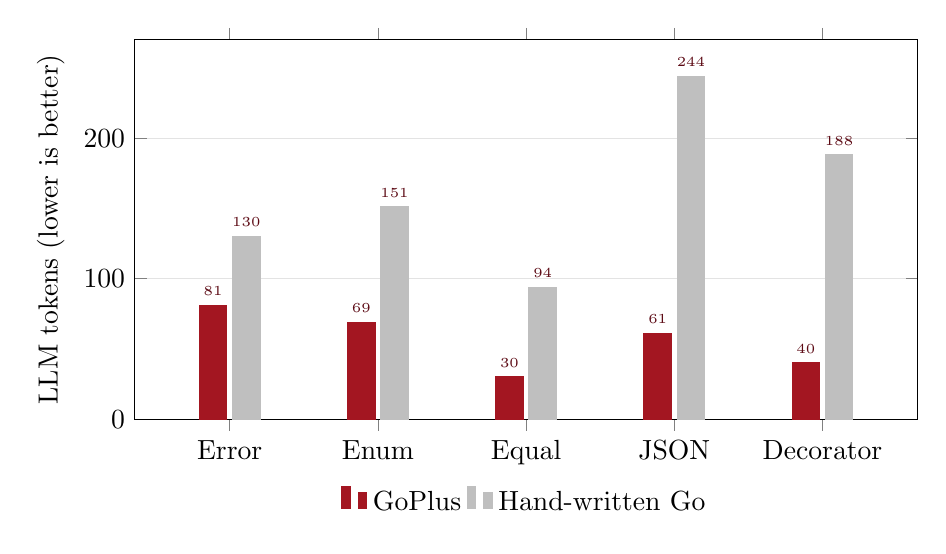
\begin{tikzpicture}
\begin{axis}[
  ybar, bar width=10pt,
  width=0.95\textwidth, height=6.4cm,
  ymin=0, ymax=270,
  ylabel={LLM tokens (lower is better)},
  symbolic x coords={Error, Enum, Equal, JSON, Decorator},
  xtick=data,
  enlarge x limits=0.16,
  legend style={at={(0.5,-0.16)},anchor=north,legend columns=-1,draw=none},
  ymajorgrids, grid style={gray!22},
  nodes near coords, nodes near coords style={font=\tiny\color{hustdark}},
]
\addplot[fill=hustred,draw=hustred] coordinates {(Error,81) (Enum,69) (Equal,30) (JSON,61) (Decorator,40)};
\addplot[fill=gray!50,draw=gray!50] coordinates {(Error,130) (Enum,151) (Equal,94) (JSON,244) (Decorator,188)};
\legend{GoPlus, Hand-written Go}
\end{axis}
\end{tikzpicture}
\caption{Tokens for the same behaviour across five patterns: GoPlus (red) versus
hand-written Go (grey). The gap widens as more boilerplate is replaced.}
\label{fig:tokens}
\end{figure}

Beyond the raw count, the GoPlus versions carry stronger guarantees: the enum
\texttt{match} is exhaustiveness-checked, whereas the equivalent hand-written Go
\texttt{switch} is not.

\subsection{Runtime parity}
Because GoPlus adds no runtime layer, its output should run exactly as fast as
hand-written Go. The same algorithm was benchmarked as GoPlus-generated Go and as
a hand-written Go equivalent, in the same package, after asserting that both
produce identical results.

\begin{table}[h]
\centering
\renewcommand{\arraystretch}{1.2}
\begin{tabularx}{\textwidth}{@{}X r r@{}}
\toprule
\textbf{Implementation} & \textbf{Time / op (median)} & \textbf{Allocations / op} \\
\midrule
GoPlus-generated Go & \(\approx\) 126\,\(\mu\)s & 0 \\
Hand-written Go     & \(\approx\) 128\,\(\mu\)s & 0 \\
\bottomrule
\end{tabularx}
\caption{The two implementations are within run-to-run noise of each other, both
with zero allocations. The enum/match sugar desugars to a plain integer
\texttt{switch}.}
\end{table}

\subsection{Decorators do real work}
The measurements so far concern GoPlus's \emph{sugar}, which should cost nothing.
Decorators are the opposite case: they exist to add behaviour and should add
exactly as much as that behaviour requires---no more. Figure~\ref{fig:memoize}
shows \texttt{@memoize} applied to a naive recursive Fibonacci: a repeated query
is answered from the cache in a few nanoseconds, versus roughly nine milliseconds
for the un-memoized recursion---a speed-up of over a million times. The point is
not the speed-up but that a single annotation delivers the cache one would
otherwise write, test, and maintain by hand.

\begin{figure}[ht]
\centering
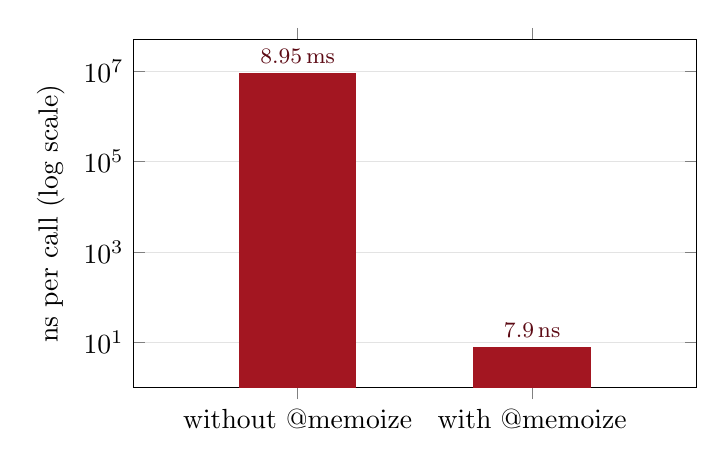
\begin{tikzpicture}
\begin{axis}[
  ybar, bar width=42pt,
  width=0.72\textwidth, height=6cm,
  ymode=log, log origin=infty,
  ymin=1, ymax=5e7,
  ylabel={ns per call (log scale)},
  symbolic x coords={without @memoize, with @memoize},
  xtick=data, enlarge x limits=0.7,
  nodes near coords, point meta=explicit symbolic,
  nodes near coords style={font=\footnotesize\color{hustdark}},
  ymajorgrids, grid style={gray!22},
]
\addplot[fill=hustred,draw=hustred] coordinates {
  (without @memoize,8948366) [8.95\,ms]
  (with @memoize,7.9) [7.9\,ns]
};
\end{axis}
\end{tikzpicture}
\caption{A repeated \texttt{fib(32)} query: without \texttt{@memoize} the naive
recursion takes \(\approx\)9\,ms; \texttt{@memoize} answers from its cache in
\(\approx\)8\,ns. Note the logarithmic scale.}
\label{fig:memoize}
\end{figure}

\subsection{Transpile speed and scaling}
Transpilation must not slow a build or CI loop. On a sample program the frontend
is microsecond-fast and code generation low-millisecond (parsing
\(\approx\)3\,\(\mu\)s, analysis \(\approx\)6\,\(\mu\)s, code generation
\(\approx\)1.4\,ms). More importantly, end-to-end transpile time scales linearly
with program size: Figure~\ref{fig:scaling} plots wall-clock time against the
number of functions, and even an 800-function source transpiles in well under a
tenth of a second. A content-hash package cache further skips packages whose
sources have not changed on rebuild.

\begin{figure}[ht]
\centering
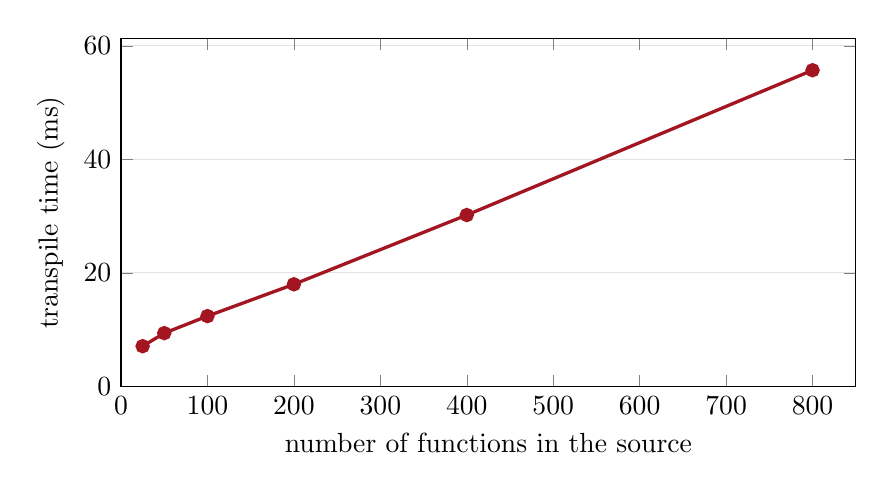
\begin{tikzpicture}
\begin{axis}[
  width=0.9\textwidth, height=6cm,
  xlabel={number of functions in the source},
  ylabel={transpile time (ms)},
  xmin=0, xmax=850, ymin=0,
  ymajorgrids, grid style={gray!22},
  mark options={fill=hustred},
]
\addplot[hustred, very thick, mark=*] coordinates {
  (25,7.1) (50,9.4) (100,12.4) (200,18.0) (400,30.2) (800,55.7)
};
\end{axis}
\end{tikzpicture}
\caption{End-to-end transpile time grows linearly with program size; an
800-function source transpiles in \(\approx\)56\,ms.}
\label{fig:scaling}
\end{figure}

\subsection{Case study: a REST service}
To test the ``readable, debuggable, review-friendly'' promise on something past a
single-file example, a small task-tracker REST service was written entirely in
GoPlus: HTTP handlers, a service layer, an in-memory store, an enum-based state
machine, and JSON serialization. The service runs, and its handlers are covered
by tests driven through the standard HTTP test harness.

The design follows a conventional three-layer shape---handlers translate HTTP to
calls, a service layer holds the business rules, and a store persists data---and
each GoPlus feature lands where it is most useful. The store returns independent
deep copies via a derived \texttt{Clone}, so a handler cannot accidentally mutate
shared state. The service validates every state change through a single
exhaustive \texttt{match}, so an illegal transition is rejected uniformly. Error
handling threads through the layers with \texttt{?}, and a logging concern is a
single decorator rather than repeated boilerplate. Request and response payloads
(de)serialize through derived JSON methods. The store is an in-memory map behind a
small set of functions; a real database driver would slot in at exactly that
boundary without touching the handlers or the service.

\begin{figure}[ht]
\centering
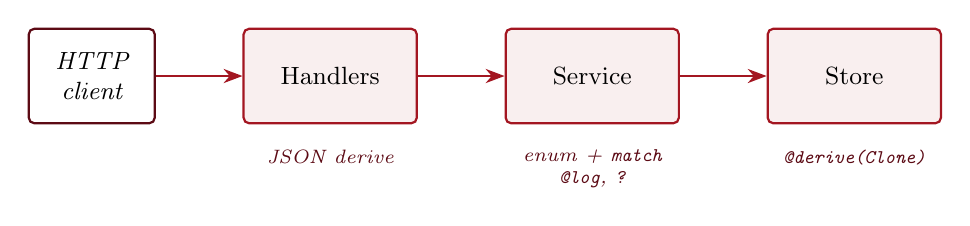
\begin{tikzpicture}[
  node distance=11mm,
  L/.style={draw=hustred,fill=hustred!7,rounded corners=2pt,thick,minimum height=12mm,
            minimum width=22mm,align=center,font=\small},
  cli/.style={draw=hustdark,fill=white,rounded corners=2pt,thick,minimum height=12mm,
              minimum width=16mm,align=center,font=\small\itshape},
  a/.style={-{Stealth[length=2.4mm]},hustred,thick},
  note/.style={font=\scriptsize\itshape\color{hustdark},align=center}]
\node[cli] (client) {HTTP\\client};
\node[L,right=of client] (h) {Handlers};
\node[L,right=of h] (s) {Service};
\node[L,right=of s] (st) {Store};
\draw[a] (client)--(h);
\draw[a] (h)--(s);
\draw[a] (s)--(st);
\node[note,below=2mm of h] {JSON derive};
\node[note,below=2mm of s] {enum + \texttt{match}\\ \texttt{@log}, \texttt{?}};
\node[note,below=2mm of st] {\texttt{@derive(Clone)}};
\end{tikzpicture}
\caption{The case-study service is layered, and each GoPlus feature lands where it
is most useful. A real database driver would replace the in-memory store without
touching the layers above it.}
\label{fig:casestudy}
\end{figure}

Two observations are worth recording. First, the layered design reads cleanly:
error flow threads through the layers with \texttt{?}, the state machine is a
single exhaustive \texttt{match}, and cross-cutting logging is one decorator.
Second---and more tellingly---building a medium-sized program exercised code
paths that single-file examples never had, and \emph{surfaced real defects in the
generated code that were then fixed}. That a case study earns its keep by finding
bugs is itself evidence that the approach scales beyond toy inputs.

\subsection{Threats to validity}
These are small, illustrative inputs measured on a single machine; the magnitudes
should be read as indicative rather than guaranteed. Token counts depend on the
chosen tokenizer and vary by model. The runtime-parity benchmark deliberately
isolates language \emph{sugar} (no decorators) to measure overhead fairly;
decorators, by design, add exactly the work they describe (a cache, a retry
loop), which is code one would otherwise write by hand.

%================================================================ 7
\section{Related Work and Positioning}
GoPlus occupies a familiar niche: a surface language that compiles to a mainstream
target while keeping the output transparent. The clearest analogy is the way a
typed surface language can compile to a widely deployed dynamic language, adding
ergonomics and static checks without introducing a new runtime; GoPlus applies
the same philosophy to Go.

Its individual features are well established in language design---error
propagation operators, algebraic enumerations with exhaustive matching, and
compile-time decorators all have mature precedents. GoPlus's contribution is not
to invent these mechanisms but to \emph{compose a carefully scoped subset of them
on top of Go while guaranteeing readable, idiomatic Go output}. In contrast to
approaches that introduce a bespoke runtime, a heavyweight type system, or opaque
macro expansion, GoPlus keeps the generated code inspectable and the language
small, which is precisely what preserves compatibility and avoids lock-in.

%================================================================ 8
\section{Discussion, Limitations, and Adoption}
\subsection{What the design buys, and what it costs}
The consistent theme across the evaluation is that GoPlus removes repetitive,
error-prone code while adding static guarantees, at no runtime cost. The cost it
does impose is a modest one: a team takes on a build step and a surface syntax
that, while close to Go, is not Go. GoPlus keeps that cost low by two deliberate
choices---accepting standard Go syntax alongside its own, and emitting readable
Go---so the barrier to trying it, and the barrier to leaving it, are both small.

\subsection{Limitations}
GoPlus is an evolving project, and several boundaries are worth stating plainly.
A handful of line-level constructs are still carried through as verbatim text
rather than fully structured, which bounds how deeply they can be analyzed.
Package-qualified decorators are not signature-checked. The richer derivations
(ordering, hashing) and user-defined derivations are not yet available. And the
evaluation, while measured on real inputs, uses small programs on a single
machine; the numbers should be read as indicative of direction and magnitude
rather than as guarantees.

\subsection{How a team would adopt it}
Because a package may mix \texttt{.gp} and \texttt{.go} files, adoption can be
incremental: a team can write one new package---or one new file---in GoPlus,
review the generated Go, and expand from there. The generated code is checked in
or produced by the build like any other artefact, and the standard Go tooling
(testing, profiling, modules) applies unchanged to it. If the experiment does not
work out, the generated Go is the exit path.

%================================================================ 9
\section{Conclusion and Future Work}
GoPlus is a productivity layer that makes everyday Go more concise and safer to
write while keeping the generated Go fully transparent. It streamlines error
flow, adds exhaustiveness-checked enumerations and pattern matching, and offers
safe compile-time decorators and derivations---backed by a coherent toolchain of
formatter, linter, diagnostics, and editor support. The evaluation indicates a
substantial reduction in the amount of code written (about 65\% fewer tokens on
the measured patterns) with no measurable runtime cost and fast transpilation,
and a medium-sized case study shows the approach holds up on a real service.

Several directions remain open. On the language and codegen side: richer
derivations (ordering and hashing), user-defined derivations, and deeper
structured parsing of the remaining line-level constructs. On the ecosystem side:
better large-project package handling, wider editor and marketplace availability,
and a broader benchmark suite tracked over time. The guiding constraint will not
change: whatever is added must still lower to Go that a person could have written
by hand.

%---------------------------------------------------------------- References
\begin{thebibliography}{9}
\bibitem{go} The Go Programming Language. \url{https://go.dev}.
\bibitem{gofmt} \texttt{gofmt} --- format Go source code. \url{https://pkg.go.dev/cmd/gofmt}.
\bibitem{effgo} \emph{Effective Go}. \url{https://go.dev/doc/effective_go}.
\bibitem{rust} The Rust Programming Language (implementation language of the transpiler). \url{https://www.rust-lang.org}.
\bibitem{mdbook} mdBook --- documentation tooling. \url{https://rust-lang.github.io/mdBook}.
\bibitem{repo} GoPlus source repository. \url{https://github.com/Trinq2003/golang-plus}.
\end{thebibliography}

\clearpage
\appendix
\section{A complete example}
The following self-contained program exercises the core surface features:
a derived enumeration, an exhaustive \texttt{match}, error propagation with
\texttt{?}, and a structured loop. It is ordinary GoPlus that compiles to plain,
\texttt{gofmt}-formatted Go.

\begin{lstlisting}[language=GoPlus,caption={A small, complete GoPlus program.}]
package main

import "fmt"

@derive(String)
enum Band { Low  Medium  High }

fn classify(score: int) -> Band! {
    if score < 0 {
        return error("score must be non-negative")
    }
    if score < 40 {
        return Band::Low
    }
    if score < 80 {
        return Band::Medium
    }
    return Band::High
}

fn label(b: Band) -> string {
    match b {
        Low    => "needs work"
        Medium => "acceptable"
        High   => "excellent"
    }
}

fn main() -> ! {
    for _, s := range []int{12, 55, 93} {
        band := classify(s)?
        fmt.Println(s, band, label(band))
    }
    return
}
\end{lstlisting}

\section{Command-line reference}
Every command accepts a \texttt{.gp} file or a package directory.

\begin{table}[ht]
\centering
\renewcommand{\arraystretch}{1.25}
\begin{tabularx}{\textwidth}{@{}l X@{}}
\toprule
\textbf{\color{hustred}Command} & \textbf{\color{hustred}Purpose} \\
\midrule
\texttt{check}     & Parse, analyze, transpile, and type-check via the Go compiler. \\
\texttt{transpile} & Emit Go (optionally with a \texttt{.gp}\,\(\leftrightarrow\)\,\texttt{.go} source map). \\
\texttt{build}     & Transpile, then build a binary. \\
\texttt{run}       & Transpile, then run. \\
\texttt{test}      & Transpile, link sibling Go and test files, then run \texttt{go test}. \\
\texttt{fmt}       & Format \texttt{.gp} in place (comment-safe), with \texttt{--check}/\texttt{--stdout} modes. \\
\texttt{lint}      & Report style and suspicious-code diagnostics without generating Go. \\
\texttt{navigate}  & Resolve a position between \texttt{.gp} and generated \texttt{.go} via a source map. \\
\bottomrule
\end{tabularx}
\caption{The GoPlus command-line interface.}
\end{table}

\end{document}
